%%%%%%%%%%%%%%%%%%%%%%%%%%%%%%%%%%%%%%%%%%%%%%%%%%%%%%%%%%%%%%%%%%%
% Method
% Team:
% Union
% Members: 
% Bernie Huang, Jim Lan, Hoang Tan, Kenny Hsu, Rahul Aditya, Tan Phat, Wei
% Relative files:
% Method_Union.tex
% Note:    
% Do not compile this file compile Main.tex to get the pdf file instead.
%%%%%%%%%%%%%%%%%%%%%%%%%%%%%%%%%%%%%%%%%%%%%%%%%%%%%%%%%%%%%%%%%%%
	
\subsection*{Title extraction}

\subsubsection*{Author extraction}


\subsubsection*{Abstract extraction}
\begin{itemize}
	\item I use the python to catch the abstract.
	\begin{center}
		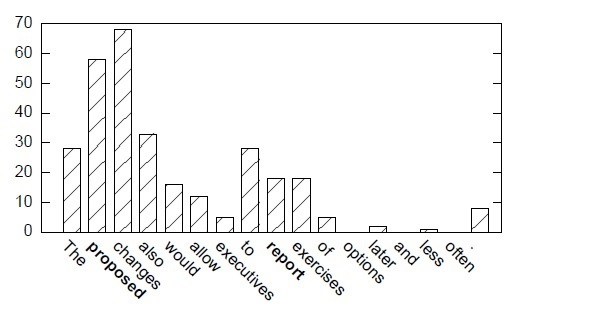
\includegraphics[width=0.8\columnwidth]{Union_Background_Chart_2}
	\end{center}
	\item Fist,the pdf is converted into txt file.Thus, it will create the txt file.\\ 
	\item Second,read the txt file on every line.If the python detects the abstract-database's words ,it will start to catch the sentences.\\ 	
	abstract-database:including the condition\\
	1. capital         "ABSTRACT"\\
	2. lower case      "abstract"\\
	3. in the sentence "Abstract—Word sense ....."\\
	4. and so on \\
	\item Third,read the txt file on every line.If the python detects the abstract-database-stop's words ,it will stop to catch the sentences.\\ 
	abstract-database-stop:including the condition
	1. the blank line
	2. specific words in the beginning "Keywords"
	3. and so on
	\item Fourth,output the sentences in the txt file\\ 	
	
\end{itemize}

\subsubsection*{Search sentences}
\begin{itemize}
	\item I use python to complete the task. 
	\begin{center}
		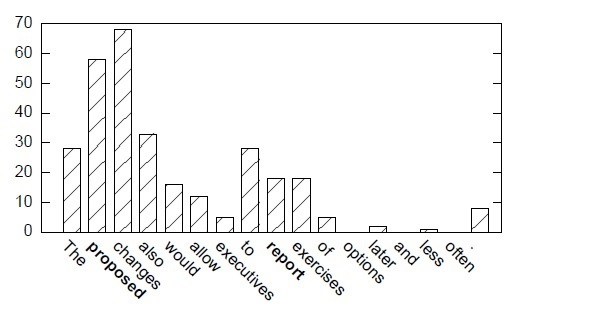
\includegraphics[width=0.8\columnwidth]{Union_Background_Chart_2}
	\end{center}
	\item First,turn the PDF to the txt file .(Make the programe easy to read file)\\ 
	\item Second,read the txt file by lines.\\ 	
	\item Third,create the array to divide the section of the articles.\\ 	
	\item Forth,expend the array to divide the section clearly.\\ 	
	\item Fifth,User search the sentence.The programe search all sections by this sentence.\\
	\item Sixth,Show the results\\  		
	
\end{itemize}

\newpage % Ends the current page and causes all figures and tables to be printed